%% ****** Start of file aiptemplate.tex ****** %
%%
%%   This file is part of the files in the distribution of AIP substyles for REVTeX4.
%%   Version 4.1 of 9 October 2009.
%%
%
% This is a template for producing documents for use with 
% the REVTEX 4.1 document class and the AIP substyles.
% 
% Copy this file to another name and then work on that file.
% That way, you always have this original template file to use.

%\documentclass[aip,graphicx]{revtex4-1}
%\documentclass[aip,reprint]{revtex4-1}

%\usepackage{graphicx}

%\draft % marks overfull lines with a black rule on the right
%\documentclass[pre,aps,floatfix,authordate1-4,twocolumn]{revtex4-1}
%\documentclass[pre,aps,floatfix,authordate1-4]{revtex4-1}

\documentclass[aps,prl,superscriptaddress,twocolumn]{revtex4}



%\documentclass[aps,prl,preprint,groupedaddress]{revtex4}

\usepackage{rotating} 
\usepackage{times}
\usepackage{graphicx}
\usepackage{setspace}
\usepackage{amsmath}
\usepackage{epstopdf}
\usepackage[obeyFinal]{easy-todo}
\usepackage{csquotes}
\usepackage{xr}


\makeatletter
\newcommand*{\addFileDependency}[1]{% argument=file name and extension
  \typeout{(#1)}
  \@addtofilelist{#1}
  \IfFileExists{#1}{}{\typeout{No file #1.}}
}
\makeatother

\newcommand*{\myexternaldocument}[1]{%
    \externaldocument{#1}%
    \addFileDependency{#1.tex}%
    \addFileDependency{#1.aux}%
}

\myexternaldocument{manuscriptPGPEsuppl}

\begin{document}

% Use the \preprint command to place your local institutional report number 
% on the title page in preprint mode.
% Multiple \preprint commands are allowed.
%\preprint{}

\title{NMRlipids IV: Headgroup \& glycerol backbone structures, and cation binding in bilayers with PE and PG lipids} %Title of paper

% repeat the \author .. \affiliation  etc. as needed
% \email, \thanks, \homepage, \altaffiliation all apply to the current author.
% Explanatory text should go in the []'s, 
% actual e-mail address or url should go in the {}'s for \email and \homepage.
% Please use the appropriate macro for the type of information

% \affiliation command applies to all authors since the last \affiliation command. 
% The \affiliation command should follow the other information.

\author{Am{\'e}lie Bacle}
\affiliation{Paris, France}

\author{Pavel Buslaev}
\affiliation{University of Jyv{\"a}skyl{\"a}}

\author{Rebeca Garc{\'i}a Fandi{\~n}o}
\affiliation{Center for Research in Biological Chemistry and Molecular Materials (CiQUS), Universidade de Santiago de Compostela, E-15782 Santiago de Compostela, Spain}
\affiliation{CIQUP, Centro de Investigação em Química, Departamento de Química e Bioquímica, Faculdade de Ciências, Universidade do Porto, Porto, Portugal}

\author{Fernando Favela-Rosales}
\affiliation{Departamento de Investigaci\'{o}n, Tecnol\'{o}gico Nacional de M\'{e}xico, Campus Zacatecas Occidente, M\'{e}xico}

\author{Tiago Ferreira}
\affiliation{Halle, Germany}

\author{Patrick Fuchs}
\affiliation{Paris, France}

\author{Matti Javanainen}
\affiliation{Institute of Organic Chemistry and Biochemistry of the 
Czech Academy of Sciences, Flemingovo n\'{a}m. 542/2, CZ-16610 Prague 6, Czech Republic}

\author{Anne M. Kiirikki}
\affiliation{Institute of Biotechnology, University of Helsinki}


\author{Jesper J. Madsen}
\affiliation{Department of Chemistry, The University of Chicago, Chicago, Illinois, United States of America}
\affiliation{Department of Global Health, College of Public Health, University of South Florida, Tampa, Florida, United States of America}

\author{Josef Melcr}
\affiliation{Institute of Organic Chemistry and Biochemistry of the 
Czech Academy of Sciences, Flemingovo n\'{a}m. 542/2, CZ-16610 Prague 6, Czech Republic}
\affiliation{Groningen Biomolecular Sciences and Biotechnology Institute 
and The Zernike Institute for Advanced Materials, 
University of Groningen, 9747 AG Groningen, The Netherlands}

\author{Paula Milan Rodriguez}
\affiliation{Paris, France}

\author{Markus S. Miettinen}
% \affiliation[Max Planck Institute of Colloids and Interfaces]{Department of Theory and Bio-Systems, Max Planck Institute of Colloids and Interfaces, 14424 Potsdam, Germany}
\affiliation{Department of Theory and Bio-Systems, Max Planck Institute of Colloids and Interfaces, 14424 Potsdam, Germany}

\author{O. H. Samuli Ollila}
\email[]{samuli.ollila@helsinki.fi}
\affiliation{Institute of Biotechnology, University of Helsinki}

\author{Chris G. Papadopoulos}
\affiliation{I2BC - University Paris Sud}


\author{Antonio Pe{\'o}n}
\affiliation{Spain}

\author{Thomas J. Piggot}
\affiliation{Chemistry, University of Southampton, Highfield, Southampton SO17 1BJ, United Kingdom}

\author{{\'A}ngel Pi{\~n}eiro}
\affiliation{Departamento de F{\'i}sica Aplicada, Facultade de F{\'i}sica, Universidade de Santiago de Compostela, E-15782 Santiago de Compostela, Spain}


% Collaboration name, if desired (requires use of superscriptaddress option in \documentclass). 
% \noaffiliation is required (may also be used with the \author command).
%\collaboration{}
%\noaffiliation

\date{\today}

\begin{abstract}
% insert abstract here
  Chemistry of lipid headgroups, the water facing components of cell membranes that regulate cell functions via lipid--protein interactions, varies between organisms and organelles. Because lipid membranes are in liquid state under physiological conditions, the conformational ensembles of different lipid headgroups are difficult to resolve experimentally. Here, we combine solid state NMR experiments and molecular dynamics simulations from NMRlipids open collaboration to resolve the conformational ensembles of the headgroups of key lipid types in liquid lamellar phase under various biologically relevant conditions. Interpretation of NMR experiments using the plethora of simulation data collected in the NMRlipids project suggests that all lipid headgroups sample a wide range of conformations in neutral and charged cellular membranes. However, the populations of different conformations are dictated by the headgroup chemistry. Together with the analysis of protein-bound lipids from the protein data bank (PDB), this suggests that lipids can bind to proteins in wide range of conformations independently on the headgroup chemistry. Therefore, the selective adsorption of proteins to membranes is likely regulated by specific protein--lipid interactions, rather than conformational restrictions of lipids. Our results pave the way to comprehensive understanding of lipid--protein interaction energetics, and the understanding of complex biomolecular assemblies such as membrane proteins.

  
\end{abstract}

%\pacs{}% insert suggested PACS numbers in braces on next line

\maketitle %\maketitle must follow title, authors, abstract and \pacs

% Body of paper goes here. Use proper sectioning commands. 
% References should be done using the \cite, \ref, and \label commands


%\label{}
\section{Introduction}

Chemical compositions of hydrophilic lipid headgroups vary between different
organelles and organisms, and different lipid types
regulate protein functions in many different ways \cite{lee03,vanmeer08}.
Lipids can directly bind to proteins or indirectly affect protein
functions by altering membrane properties such as charge or elasticity \cite{lee03,lemmon08}.
While the specific interactions with certain lipid headgroups
are known to be essential for the function of several proteins \cite{lee11,lemmon08},
it is not clear if the specificity is driven by the differences in accessible
conformational states between lipid types or
by specific intermolecular lipid--protein interactions.

The conformational ensembles of lipids in the physiologically relevant lamellar liquid phase
are typically derived from NMR experiments, particularly from 
C--H bond order parameters measured using $^2$H NMR~\cite{seelig77c,davis83,Semchyschyn04}. Notably, such measurements can be performed also on living cells \cite{gally81,scherer87,seelig90}.
These studies suggest that the glycerol backbone conformations are largely similar irrespectively of the headgroup \cite{gally81}, 
and the headgroup conformations are similar in  phosphatidylcholine (PC), phosphatidylethanolamine (PE) and phosphatidylglycerol (PG) lipids, while the headgroup is more rigid in phosphatidylserine (PS) lipids \cite{wohlgemuth80,buldt81}. 
However, these tendencies are based only on the absolute values, whereas
the necessity of order parameter signs in capturing the conformational ensembles of lipids has been recently demonstrated \cite{botan15,ollila16,ferreira16}.
Furthermore, the detailed understanding of lipid conformational ensembles
is limited by the lack of universal models that would map order parameters to structural ensembles \cite{pezeshkian18,akutsu20}.

Stuctures of different lipid types in protein bound states can be extracted from the protein data bank (PDB) \cite{berman00},
but their relation to the conformational ensembles in liquid lamellar state remains unclear \cite{marsh13b}.
In addition to the changes in lipid conformational ensembles upon binding to proteins,
also the experimentally measured response of lipid headgroup to membrane bound charges remains poorly understood 
due to the lack of suitable models to interpret the lipid conformational ensembles in liquid lamellar state \cite{Semchyschyn04}.


Here, we use natural abundance $^{13}$C NMR experiments and MD simulations from the NMRlipids open collaboration
to resolve the differences in conformational ensembles between PC, PE, PG and PS lipid headgroups.
Zwitterionic PC and PE are the most common lipids in eukaryotes and bacteria, respectively \cite{vanmeer08,sohlenkamp16}.
PE is also the second most abundant glycerophospholipid in eukaryotic cells
and has been related to various diseases \cite{vance15,calzada16,patel17}.
PS and PG are the most common negatively charged lipids in eukaryotes and bacteria, respectively,
and affect membrane protein functionality and signaling \cite{lemmon08,leventis10,sohlenkamp16,hariharan18}.
All the studied lipids specifically bind to various proteins \cite{yeagle14}. We use our results to elucidate also lipid--protein interactions and the effect of charges on lipid conformations.

The lipid conformational ensembles in liquid lamellar state paves the way toward understanding the
specific binding of different lipid types to membrane proteins and how they regulate the protein function.
Because glycerol backbone and headgroup structures of PC lipids are similar in model membranes and in bacteria \cite{gally81,scherer87,seelig90},
the results from model systems could be used to understand the biological role of lipid headgroup conformational ensembles in different lipid types.



\section{Methods}
\subsection{Experimental C--H bond order parameters}
The headgroup and glycerol backbone C--H bond order parameters of 1-palmitoyl-2-oleoyl-sn-glycero-3-phosphoethanolamine (POPE) and 1-palmitoyl-2-oleoyl-sn-glycero-3-phospho-(1'-rac-glycerol) (POPG), purchased from Avanti polar lipids, were measured using natural abundance $^{13}$C solid state NMR spectroscopy as described previously \cite{ferreira13,ferreira16}. The magnitudes of order parameters were determined from the chemical-shift resolved dipolar splittings using a R-type Proton Detected Local Field (R-PDLF) experiment~\cite{dvinskikh04} and the signs from S-DROSS experiments~\cite{gross97} combined with SIMPSON simulations \cite{bak00}.
%The experiments were done in a Bruker Avance III 400 spectrometer operating at a $^1$H Larmor frequency of 400.03 MHz.
%Magic angle spinning (MAS) of the sample was used at a frequency of 5.15 kHz (R-PDLF experiment) and 5 kHz (S-DROSS experiment).
The NMR experiments were identical as in our previous work~\cite{antila19}. The POPE experiments were recorded at 310~K and POPG experiments at 298~K, where the bilayers are in the liquid disordered phase \cite{marsh13}.

Glycerol backbone peaks from both lipids, and $\alpha$-carbon peak from POPE in the INEPT spectra 
were assigned based on previously measured POPC spectra~\cite{ferreira13}.
The $\beta$-carbon peak from POPE was assigned based on $^{13}$C chemical shift table for amines available
at \url{https://www.chem.wisc.edu/areas/reich/nmr/c13-data/cdata.htm}.
\todo{How were $\alpha$ and  $\gamma$-carbon peaks assigned in POPG?}.
The $\beta$-carbon peak from POPG overlapped with the g$_2$ peak from glycerol backbone
because their chemical environments are similar.
\todo{Details to be checked by Tiago}.

\subsection{Molecular dynamics simulations}

Molecular dynamics simulation data were collected and analyzed using
the methods from the NMRlipids Open Collaboration project (\url{nmrlipids.blogspot.fi}) \cite{botan15,catte16,ollila16,antila19}.
%\url{github.com/NMRlipids/NMRlipidsIVotherHGs}. 
Simulation and accessibility details of more than 70 systems simulated for this work are given in the supplementary information. Quality evaluation of these simulations enables us to select the best models for the interpretation of lipid conformational ensembles from the experimental data.

The quality of lipid headgroup and glycerol backbone conformational ensembles in PE and PG simulations were evaluated using the C-H bond order parameters \cite{botan15}. Interactions between different headgroups in simulations of mixed bilayers were evaluated monitoring the changes in headgroup order parameters upon mixing the lipids \cite{antila19}. The ion binding affinities and response of lipids to bound charge were evaluated monitoring the changes of lipid headgroup order parameters \cite{catte16,antila19}.


%\clearpage
\begin{figure*}[]
  \centering
%  \includegraphics[width=9.0cm]{../Figs/lipids.pdf}
  %  \includegraphics[width=9.0cm]{../Figs/HGorderparametersPCPSPEPG.eps}
   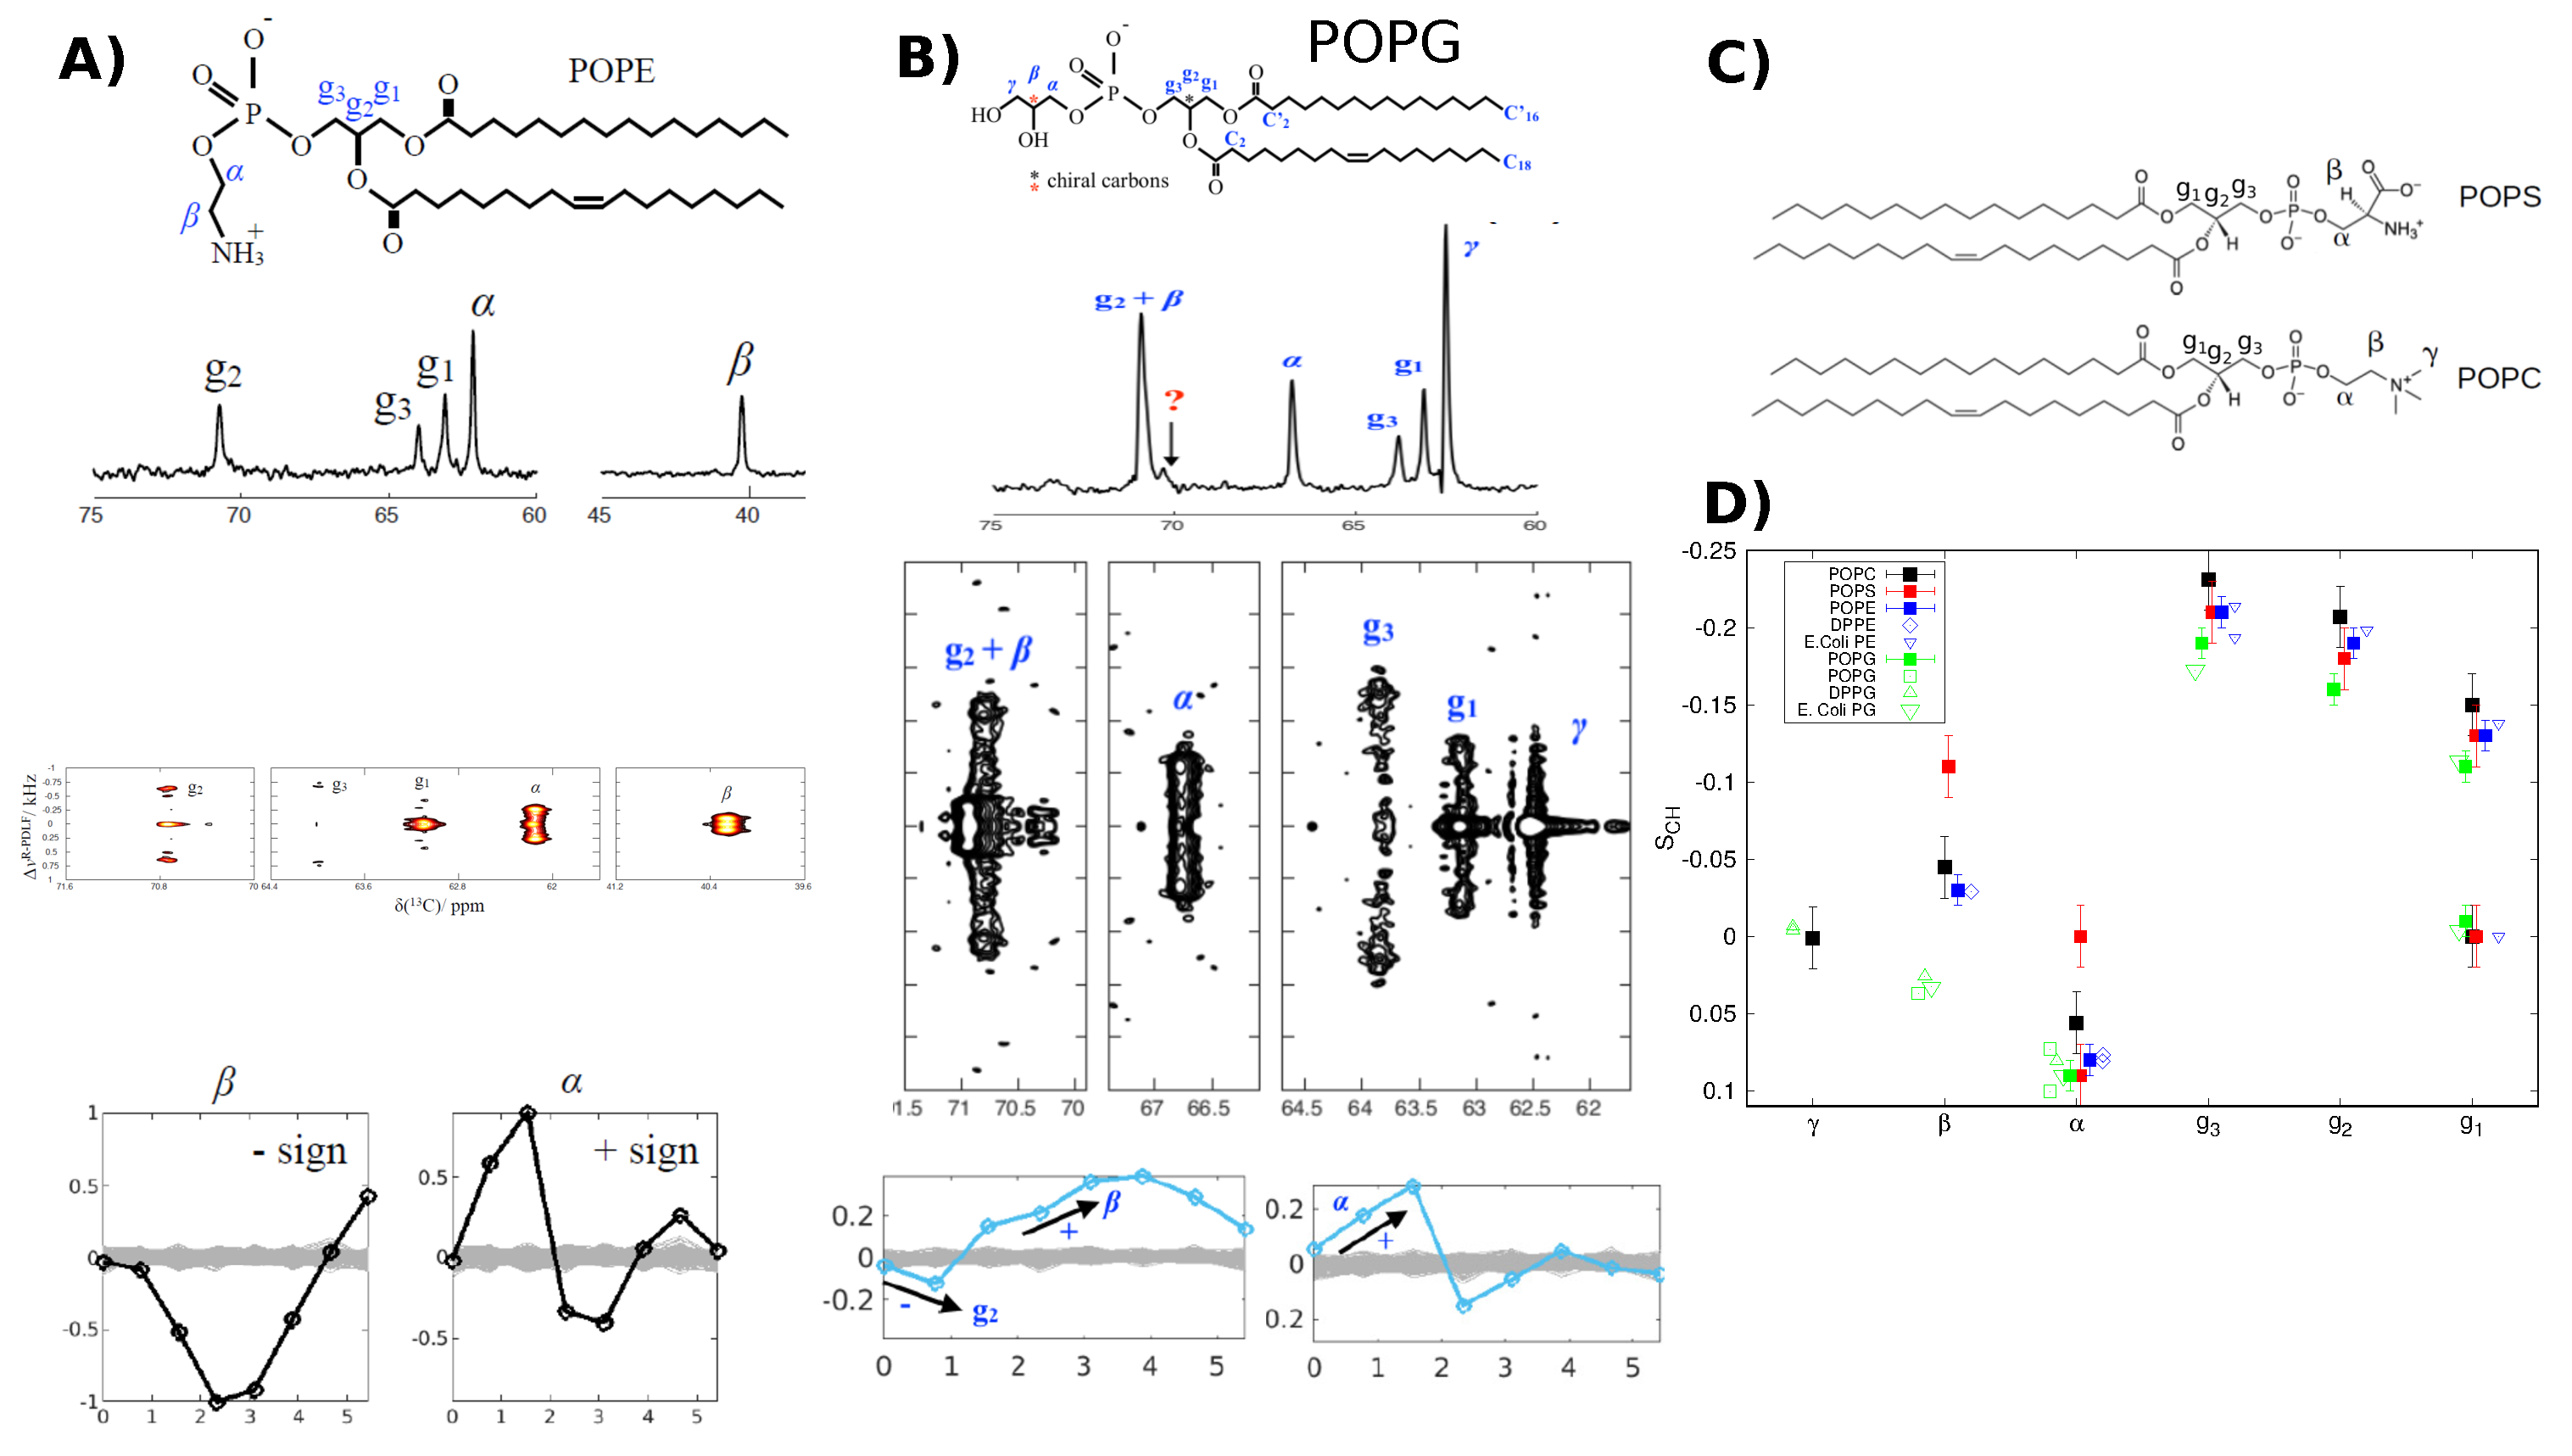
\includegraphics[width=18.0cm]{./Figs/figure1.eps}
   \caption{\label{HGorderParameters}
     Chemical structure, refocused-INEPT spectrum, 2D R-PDLF spectra, and S-DROSS data (from top to bottom) of \textbf{A)} POPE  and \textbf{B)} POPG.
      Full NMR spectra are shown Figs. \ref{POPEspectra} and \ref{POPGspectra}.
     \textbf{C)} Chemical structure of POPC and POPS.
    \textbf{D)} Headgroup and glycerol backbone order parameters from different experiments in lamellar liquid disordered phase.
    The values and signs for POPE (310~K) and POPG (298~K)
    measured in this work, and for POPS (298~K) \cite{antila19} and POPC (300~K) \cite{ferreira13,ferreira16}
    previously using $^{13}$C NMR. The literature values for
    DOPS with 0.1M of NaCl (303~K) \cite{browning80},
    POPG with 10nM PIPES (298~K) \cite{borle85},
    DPPG with 10mM PIPES and 100mM NaCl (314~K) \cite{wohlgemuth80}, 
    DPPE (341~K) \cite{seelig76},
    E.coliPE and E.coliPG (310~K) \cite{gally81}
    are measured using $^2$H NMR. The signs from $^{13}$C NMR are used also for the literature values.
   }
   \todo{This is a sketch, Tiago Ferreira will make a new figure.} \\
%  \todo{D) could be clarified as Fig. 2 in the NMRlipids IVps paper.}
\end{figure*}


\subsection{Analysis of conformations of protein-bound lipids}
\todo{This is to be finished once the final analysis is done as discussed in this issue: https://github.com/NMRLipids/NMRlipidsIVPEandPG/issues/40}

Lipid structures from Protein Data Bank (PDB, \url{http://www.rcsb.org/})
were searched using PDBe REST API (\url{www.ebi.ac.uk/pdbe/pdbe-rest-api}).
First, all PDB entries containing PC, PE, PG, or PS lipid headgroups were collected.
The ligand names to identify the lipids were:
PLC, PX4, 6PL, LIO, HGX, PC7, PC8, P1O, 6O8, XP5, EGY, PLD, SBM, HXG, and PCW for PC;
8PE, PTY, 3PE, PEH, PEF, 6OE, 6O9, 9PE, PEV, 46E, SBJ, L9Q, PEK, EPH, ZPE, 9TL, 9Y0, 6OU, LOP, and PEE for PE;
PGT, PGK, LHG, 44G, PGV, OZ2, D3D, PGW, DR9, P6L, PG8, H3T, and GOT for PG; and
PSF, PS6, Q3G, P5S, D39, PS2, 17F, and 8SP for PS.
Secondly, all PDB structures containing these ligands were downloaded and the dihedral angles of the first lipid in the latest version of the structures within each PDB code were calculated using the MDTraj python library \cite{mcgibbon15}.
The used Jupyter notebook is available from the project's GitHub repository (\textit{ scripts/pdbSEARCH.ipynb}).



\section{Results and Discussion}

\begin{figure*}[bt]
  \centering
   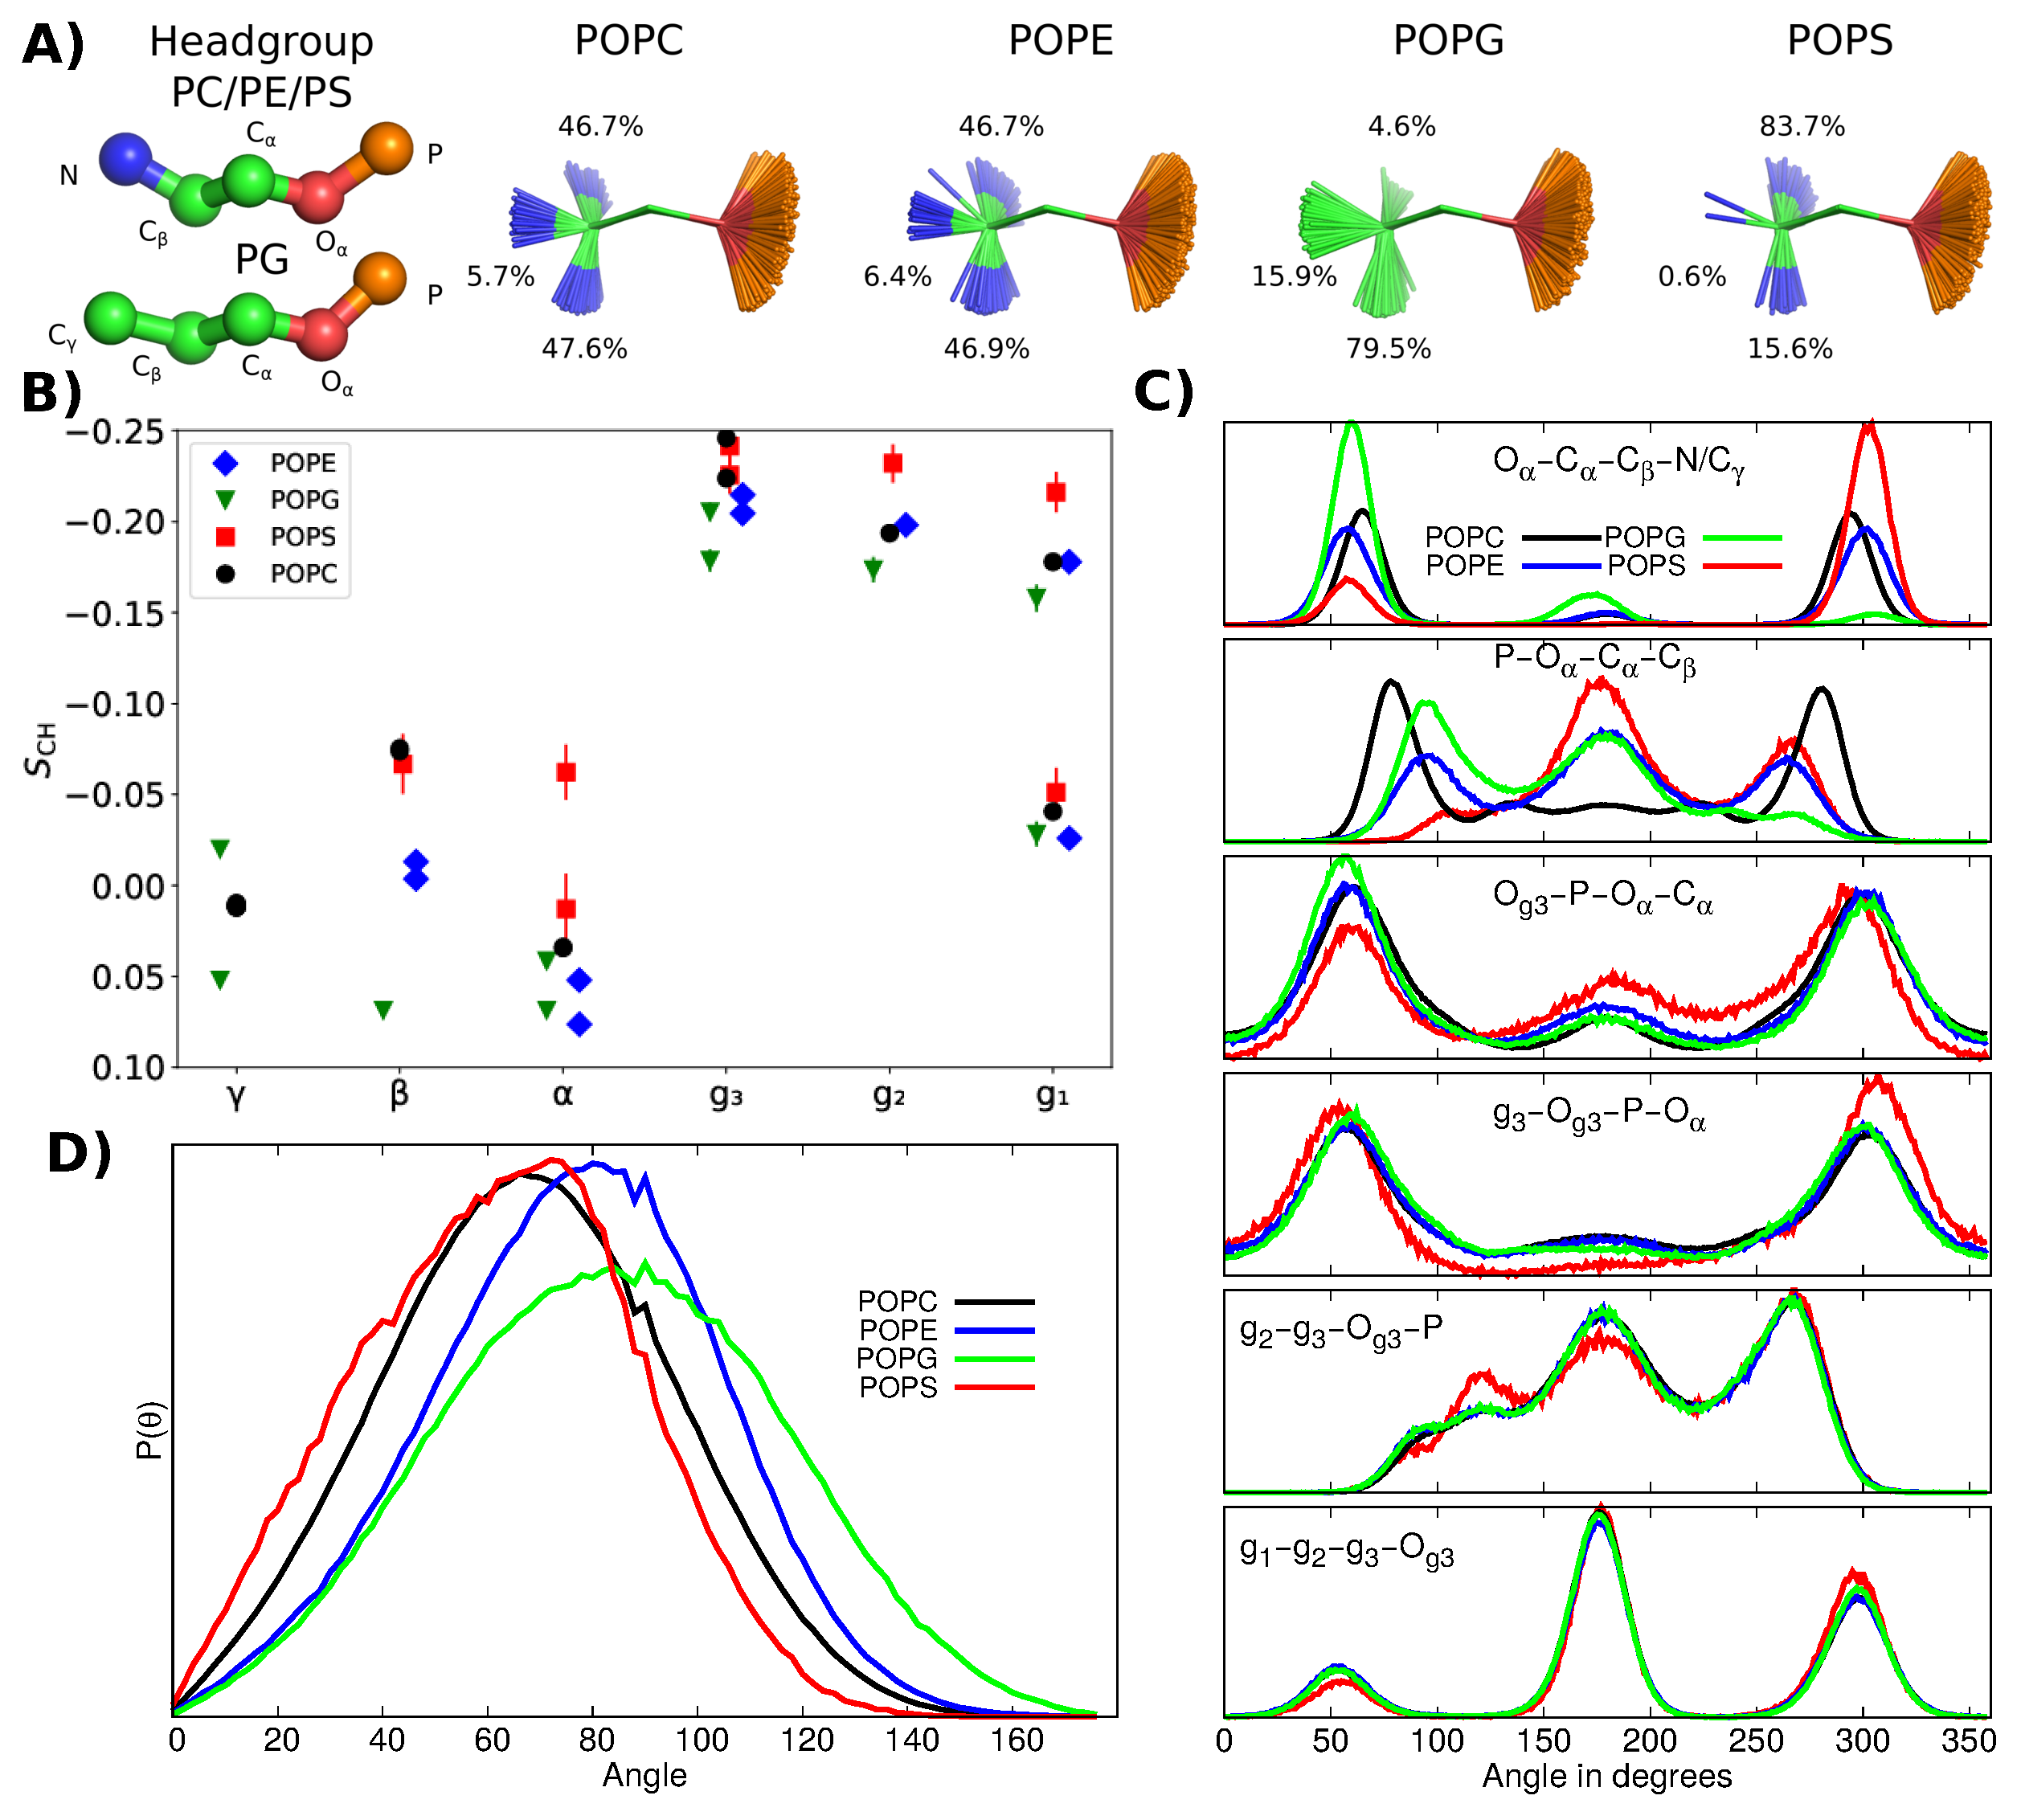
\includegraphics[width=18.0cm]{./Figs/figure2.eps}
   \caption{\label{structures}
     Results from the best simulation model (CHARMM36) simulations demonstrating the differences in conformational ensembles between different lipids. 
     \textbf{A)} Snapshots with overlayed C$_\beta$, C$_\alpha$ and O$_\alpha$ atoms and occurence of different conformations.
     \textbf{B)} Headgroup and glycerol backbone region order parameters of different different lipids.
     \textbf{C)} Distributions of heavy atom dihedral angles of different lipids from simulations.
     \textbf{D)} Distributions of P-N vector angle with respect to membrane normal.
  }
\end{figure*}


\subsection{Differences between lipid headgroups in bulk bilayer from $^{13}$C NMR experiments}

To experimentally characterize the headgroup conformational ensembles of lipids that are not bound to proteins in an electrostatically neutral cell membrane, we measured the C--H bond order parameters and their signs of POPG and POPE in the liquid lamellar phase, as we did previously for POPC and POPS \cite{ferreira13,ferreira16,antila19}.
Determination of headgroup and glycerol backbone order parameters and their signs
was straightforward from the data in Figs.~\ref{HGorderParameters}, \ref{POPEspectra} and \ref{POPGspectra}
for all the C--H bonds, except for the $\beta$ and g$_2$ carbons in POPG.
These carbons have overlapping peaks in the INEPT spectra due to their similar chemical environments,
and only the magnitude of the larger order parameter could be determined from the R-PDLF spectra (Fig.~\ref{HGorderParameters}B)).
Nevertheless, based on previous $^2$H NMR measurements \cite{wohlgemuth80,gally81,borle85},
we assigned the larger order parameter to the g$_2$ carbon
and used the literature value for the $\beta$-carbon in SIMPSON simulations to determine the signs.
The decrease in the beginning of the S-DROSS curve suggests that the sign of larger g$_2$ order parameter
is negative and later increase suggests that sign of smaller $\beta$ order parameter is positive (Fig.~\ref{HGorderParameters}B)).
This interpretation is confirmed by SIMPSON calculations in Fig.~\ref{POPGsimpson}.

Experimental order parameters of POPC, POPE, POPG and POPS glycerol backbones and headgroups from this and previous studies are collected in Fig.~\ref{HGorderParameters}D), where signs determined from $^{13}$C NMR experiments are used also for the $^2$H NMR data from the literature. The overall agreement of order parameters determined by different research teams and different techniques for the same lipid headgroup is very good here and in previous studies \cite{botan15,ollila16,antila19}. This suggests that the observed differences between lipid types arise from differences in headgroup chemistry rather than inaccuracies in experiments, or differences in the acyl chains or in experimental conditions. The most distinct order parameters are observed for PS headgroups, for which the $\alpha$-carbon order parameter exhibits significant forking and the $\beta$-carbon has more negative value than other studied lipid types. On the other hand, the $\beta$-carbon order parameter of PG headgroup has a positive sign, in contrast to all the other lipid types. Notably, this has not been observed in traditional $^2$H NMR experiments, where only the absolute value of the order parameters are measured~\cite{wohlgemuth80,gally81,borle85}. The glycerol backbone order parameters are similar for all the lipid types, although they move slightly toward positive values (closer to zero) in the order PC $<$ PE $<$ PS $<$ PG. Essential differences between PC and PE headgroups are not observed.

\subsection{Conformational ensembles of different lipid headgroups in bulk bilayer from MD simulations}

\begin{figure*}[bt]
  \centering
  \includegraphics[width=18.0cm]{./Figs/HGorderparametersPCvsSURFchangeDIHEDRALS.eps}
  \caption{\label{changesWITHsurf}
    \textbf{A)} Modulation of PC headgroup order parameters and P--N vector angle upon addition of cationic surfactant
    from CHARMM36 simulations compared with the experimental data \cite{scherer89}.
    \textbf{B)} Changes in PC headgroup conformational ensembles upon increasing the amount of positive charge in bilayer,
    characterized by the heavy atom dihedral distributions, from CHARMM36 simulations.
  }
\end{figure*}

%To resolve the conformational ensembles of lipid headgroups, we compared the headgroup and glycerol backbone C--H bond order parameters from different MD force fields to the experimental data. 
%Although none of the simulations reproduce the headgroup order parameters within experimental accuracy for any of the analysed lipids (Figs.~\ref{HGorderParametersPE} and \ref{HGorderParametersPOPG} in the SI and Refs. \cite{botan15,antila19}), the CHARMM36 
%force field performs best for all the headgroups and 
%simulations reproduce the experimentally observed distinct order parameters of PS and PG lipids (Fig.~\ref{structures}B). 
To understand the structural origin of distinct order parameters for PG and PS lipids, we selected the simulations that best reproduce the differences between headgroups (based on the quality evaluation in the SI and Refs. \cite{botan15,antila19}) and calculated the distributions of heavy atom dihedral angles from simulations, shown in Fig.~\ref{structures}C. Major differences between headgroups are observed for the last two dihedrals in the headgroup end,  O$_\alpha$-C$_\alpha$-C$_\beta$-N/C$_\gamma$ and P-O$_\alpha$-C$_\alpha$-C$_\beta$, which prefer \textit{gauche$^-$} conformations for PG and \textit{gauche$^+$} for PS. Rest of the dihedrals are similar between different lipids, with the exception of PS lipids for which distinct distributions are observed particularly around phosphate group. Therefore we suggest that the main differences between lipid headgroups leading to distinct order parameter occur in the choline part, while also changes in phosphate region may contribute in PS lipids. This may explain the more rigid headgroup structures in PS~\cite{browning80,buldt81}. Furthermore, the angle between headgroup dipole and membrane normal decreases in the order of PG $>$ PE  $>$ PC  $>$ PS (Fig.~\ref{structures}D)). However, the differences between PC and PE in P-O$_\alpha$-C$_\alpha$-C$_\beta$ dihedral
and P--N vector dipole may be artificial as the $\beta$-carbon order parameter in PC is too negative in the CHARMM36 force field, thereby not being equal to the order parameter in PE as observed in experiments \cite{botan15}.

All lipid headgroups sample very broad conformational ensembles in liquid lamellar phase and sampled dihedral angles are within approximately same ranges for all headgroup types (Fig. \ref{structures}). The results suggest that all lipid headgroups are very flexible---thereby being able to adopt wide range of multiple conformations when interacting with proteins, ions or other biomolecules. Our results support the models that propose free rotation around phosphate group for PC lipids, which decouples the dynamics and conformations between acyl chains and headgroups \cite{klauda08c,antila21b}, and suggests that these models could be applied for all lipids containing the phosphorus group. The wide range of observed conformations suggest that the structures in lipid crystals \cite{buldt81,pascher92} play only a minor role, and that the models aiming to explain NMR data using only few conformations \cite{seelig77c,davis83,Semchyschyn04,akutsu20} are not sufficient to capture the large conformational space of lipids in liquid lamellar state.


\subsection{Lipid conformational ensembles in lipid bilayers with bound ions}

Charged entities, such as lipids, proteins, surfactants, drugs, and ions incorporated in membranes reorient the headgroup dipole in PC lipids, thereby affecting the order parameters of lipid headgroups \cite{seelig87}. However, detailed understanding on lipid conformational ensembles in membranes bearing electric charge is still lacking \cite{Semchyschyn04}.

To resolve lipid headgroup conformational ensembles in cell membrane bearing positive charge, we analyzed the simulations (CHARMM36) that correctly capture the experimentally measured decrease in PC headgroup order parameters upon addition of cationic surfactants into a bilayer in figure \ref{changesWITHsurf} A). Heavy atom dihedral angle distributions in figure \ref{changesWITHsurf} B reveal that the decrease of trans state probabilities in g$_2$-g$_3$-O$_{g_3}$-P and g$_3$-O$_{g_3}$-P-O$_\alpha$
dihedrals are the major effects of positive charge on lipid headgroup conformations. Choline region remains essentially unchanged and only minor changes are observed in other dihedrals even though almost half of the molecules in membranes are cationic surfactants. 

Also binding of ions may affect the lipid headgroup conformational ensembles in physiological conditions. In line with the results from cationic surfactants, the decreased probability for the trans state of g$_3$-O$_{g3}$-P-O$_\alpha$ dihedral is the main structural consequence of
bound Ca$^{2+}$ ion to PC headgroup (Fig.~\ref{DIHSwithCAlipid17eccPOPC} and \ref{DIHSwithCAcharmm36POPC}) in the most realistic MD simulations models (lipid17ecc and CHARMM36 in Fig.~\ref{changesWITHCaClPG}).
%Lipid17ecc (having the most realistic response of PC lipid headgroup order parameters to the calcium binding in Fig.~\ref{changesWITHCaClPG}) and CHARMM36 simulations. 
%Response of charged lipids to the ion binding is less well understood and more difficult to capture in MD simulations \cite{antila19,melcr20}.
The most realistic simulations suggest
%istic response of PG $\beta$-carbon to CaCl$_2$  even thought the calcium binding affinity was overestimated in these models.
%These models suggest
that the upward tilting of the headgroup dipole upon addition of CaCl$_2$ is weaker in PG than in PC headgroup,
%(\ref{changesWITHCaClPG}),
but dihedral distributions are more sensitive to the bound ions in PG (Lipid17 and Slipids in Figs.~\ref{changesWITHCaClPG},~\ref{DIHSwithCAslipidsPOPG} and \ref{DIHSwithCAlipid17POPG}).
However, the changes in dihedrals upon addition of calcium differ between the best models (Figs.~\ref{DIHSwithCAslipidsPOPG} and~\ref{DIHSwithCAlipid17POPG}), none of the simulations captures the calcium binding affinity and conformational ensemble of PG lipids simultaneously, and experimental data to evaluate the response of $\alpha$-carbon order parameters to the added calcium in PG is not available. Also the lipid headgroup conformational ensembles in mixed PC:PE and PC:PG membranes were not possible to resolve with the currently available force fields and experimental data (Figs.~\ref{HGorderparametersPCvsPEPG} and~\ref{HGorderparametersPGvsPCchange}).

%Therefore, more accurate force fields are required for the detailed analysis of the interactions between ions and charged lipids, as concluded previously also for PS lipids \cite{antila19,melcr20}.

Despite the 
%limited capability of simulations to interpret some of the experimental data due to the 
inaccuries in simulations in some cases, we can conclude that the experimentally observed changes in headgroup order parameters upon addition of charges into bilayer arise from relatively small changes in conformational ensembles. These changes eventuate from mild changes in dihedral angle distributions, rather than from restriction of lipids into
fixed conformations. Therefore, lipid headgroups remain in disordered state sampling large space of different conformations, thereby being able to interact with different molecules in various ways, also in membranes bearing electric charge.



\subsection{Protein-bound lipid conformations}

To analyze the alterations in lipid conformations when bound to proteins,
we calculated the heavy atom dihedral distributions from lipid conformations within protein structures deposited in the PDB \cite{berman00} in Fig.~\ref{dihedralsFROMpdb}.
\todo{This part is to be finished once the analysis if finalized}
We found 176 PC, 198 PE, 70 PG, and 41 PS conformations, which
present lipids that are tightly bound to proteins in fixed conformations
that can be determined as a part of protein structure using crystallography or cryo-EM. 


\begin{figure}[]
  \centering
  \includegraphics[width=8.0cm]{./Figs/DIHEDRALSALLfromPDB.eps}
%  \includegraphics[width=8.0cm]{../Figs/DIHEDRALSPEfromPDB.eps}
%  \includegraphics[width=8.0cm]{../Figs/DIHEDRALSPGfromPDB.eps}
%  \includegraphics[width=8.0cm]{../Figs/DIHEDRALSPSfromPDB.eps}
  \caption{\label{dihedralsFROMpdb}
    Dihedral distributions from simulations and lipid structures in PDB.
  }
\end{figure}

Similarly to the liquid lamellar state, lipid dihedrals have very wide range of angles
when bound to proteins. Only %restrictions seem to be in 
P-O$_\alpha$-C$_\alpha$-C$_\beta$ and g$_2$-g$_3$-O$_{g_3}$-P dihedrals
seem to avoid $cis$ conformations as observed also in liquid lamellar state.
The %range of available angles for
O$_\alpha$-C$_\alpha$-C$_\beta$-N/C$_\gamma$ and
g$_1$-g$_2$-g$_3$-O$_{g_3}$ dihedrals are even less restricted in protein bound state
than in liquid lamellar phase where $cis$ and $anti$ eclipsed state were not present (Fig.~\ref{structures}). 
Major differences between different lipid headgroups are not observed when bound to proteins.
Slight preference for the trans state in O$_\alpha$-C$_\alpha$-C$_\beta$-/C$_\gamma$ dihedral of PC,
and for positive angles in P-O$_\alpha$-C$_\alpha$-C$_\gamma$ dihedral of PS lipids with respect
to other lipids could be present in the data, but the statistics is not sufficient for conclusions.
Therefore, the differences in conformational ensembles between different
lipids in liquid lamellar state in Fig.~\ref{structures} are not seen in the protein bound states.

This suggests that lipids can bind to proteins in wide range of conformations independently
of headgroup chemistry. Thereby, lipids compromise their preferred conformations when binding
to proteins and the binding of lipids to specific locations would be driven by 
the intermolecular interactions between proteins and lipids.
However, it is important to note that lipids are often not the main target in
structures deposited in PDB and therefore their conformations may be less reliable than those of proteins.
Stereochemical violations and structures deviating from lipid crystals have been
previously proposed to indicate inaccuracies in lipid structures in PDB \cite{marsh13b,pezeshkian18}. 
However, we see large deviations from lipid crystals structures also in conformational ensembles
that reproduce the NMR data in liquid lamellar phase, thereby proposing that such deviations
are realistic also in protein-bound states.

\section{Conclusions}

Conformational ensembles resolved using solid state NMR experiments and MD simulations
from NMRlipids open collaboration revealed that headgroups of the most abundant biological
phospholipids, PC, PE, PG and PS, sample a wide range of different conformations in the lamellar liquid state.
Differences in NMR order parameters between different headgroups can be explained
by the changes in dihedral angle distributions, suggesting that
similar conformations are accessed by all headgroups, but with different probabilities.
Also the changes in order parameters upon the addition of charged molecules---such as cationic lipids, surfactants, or drugs---in membranes can be explained by the changes in dihedral angle probabilities, particularly close to the phosphate region.

Wide range of conformations are observed also in lipids that are tightly bound to proteins in PDB,
suggesting that the specific binding of lipids to proteins is dominated by the intermolecular lipid--protein
interactions, while the differences in conformational ensembles between different lipid types
play a minor role. Therefore, lipids can conform themselves to multiple binding positions located
in various proteins.

Our results pave the way to understanding how lipids regulate membrane protein function.
Lipid conformational ensembles in liquid lamellar phase are necessary
for the detailed analysis of lipid--protein interaction energetics, particularly for its entropic component. 
Furthermore, our results demonstrate how the NMRlipids databank, containing MD simulations and NMR data,
can be used to resolve conformational ensembles of disordered biomolecules in a membrane environment,
and how this information can be coupled with structural data in the PDB.
We believe that this combination brings us closer to the comprehensive understanding of
complex biomolecular assemblies containing both disordered and structural regions, such as membrane
protein complexes.

% If you have acknowledgments, this puts in the proper section head.
\begin{acknowledgments}
AP is grateful to the Centro de
Supercomputación de Galicia (CESGA) for use of the Finis
Terrae computer
    %     Put your acknowledgments here.
\end{acknowledgments}


% Create the reference section using BibTe
\bibliography{refs.bib}

%\newpage
%\section{APPENDIX: The NMR results reported by Tiago Ferreira}

\listoftodos

\end{document}
%
% ****** End of file aiptemplate.tex ******
